\section{Introduction}
Ice sheet dynamics are fairly well understood and, thus, models simulating ice sheet physics are fairly standard. Ice sheet models are now used as part of larger Earth System Models or as the model core to investigate interactions with their surroundings such as basal erosion. 

GLIMMER\footnote{GLIMMER used to be an acronym the meening of which has long been lost. It should no be considered to be a nice name.} is a set of libraries, utilities and example climate drivers used to simulate ice sheet evolution. Its design is motivated by the desire to create an ice modelling system which is easy to interface to a wide variety of climate models, without the user having to have a detailed knowledge of its inner workings. This is accomplished by providing a very well-defined interface, which allows access to all the functionality required by the user.

\subsection{Overview}
GLIMMER consists of
\begin{enumerate}
\item {\bf GLIDE:} {\bf G}eneral {\bf L}and {\bf I}ce {\bf D}ynamic {\bf E}lements, the core of the model.  This component is the actual ice sheet model. GLIDE is responsible for calculating ice velocities, internal ice temperature distribution, isostatic adjustment and melt water production.
\item {\bf SIMPLE:} EISMINT climate drivers.
\item {\bf GLINT:} {\bf G}ENIE {\bf I}nterface. Coupler for the GENIE\footnote{Grid-ENabled Integrated Earth-system model} Earth Systems Model.
\item {\bf EIS:} {\bf E}dinburgh {\bf I}ce {\bf S}heet climate driver based on a parameterisation of the equilibrium line altitude, sea--level surface temperatures and eustatic sea--level change.
\item {\bf GLUM:} {\bf G}Limmer {\bf U}seful {\bf M}odules, various utility procedures used by the other components.
\item Visualisation programs using GMT\footnote{Generic Mapping Tools}.
\end{enumerate}
\begin{figure}[htbp]
  \centering
  \epsfig{file=\dir/figs/glimmer.eps,width=0.6\textwidth}
  \caption{Relationship between the various GLIMMER components.}
  \label{ug.fig.glimmer}
\end{figure}
The relationship between the GLIMMER components is illustrated in Figure \ref{ug.fig.glimmer}.

\subsection{Climate Drivers}
The core ice sheet model, GLIDE, is connected to the climate via the surface mass balance and temperature fields and (optionally) a scalar value for eustatic sea level. These drivers can be derived from simple assumptions, e.g. uniform mass balance or EISMINT tests, or from climate model output, e.g. GENIE or a regional climate model. These components and how their relations are outlined in Figure \ref{ug.glide}.

\begin{figure}[htbp]
 \begin{center}
   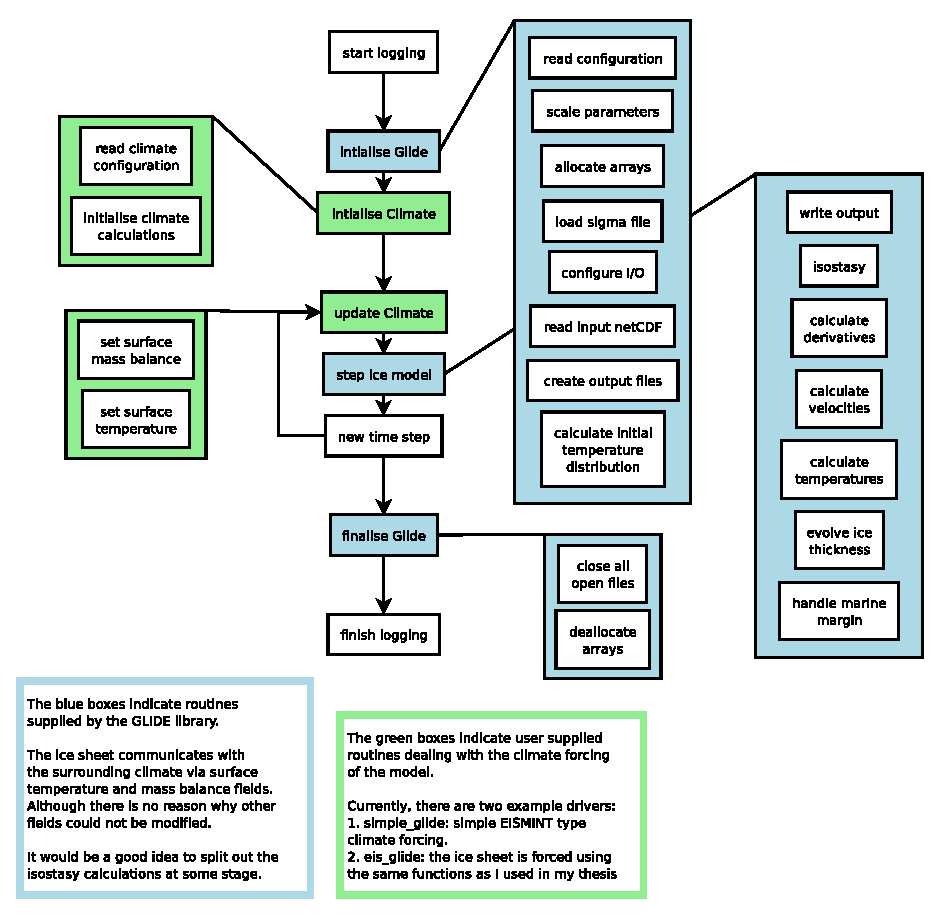
\epsfig{file=\dir/figs/glide.eps,width=0.9\textwidth}
 \end{center}
 \caption{Outline of the GLIDE and Climate components.}
\label{ug.glide}
\end{figure}

\subsection{Configuration, I/O and Visualisation}
Each component is configured using a configuration file similar to Windows \texttt{.ini} files. The model configuration is printed to a log file. 

2D and 3D data is read/written to netCDF files using the CF convention. netCDF is scientific data format for storing multidimensional data in a platform and language independent binary data format. The CF conventions specify the meta data used to describe the file contents.

Many programs can process and visualise netCDF data, e.g. OpenDX. Additionally, the GLIMMER module contains GMT scripts written in Python to visualise the output.

\subsection{Can I use GLIMMER with my climate model?}
We hope so! The external interface of GLIMMER is designed to be quite
flexible, but certain assumptions have necessarily been made about the form
taken by input fields, etc. Check out the climate drivers for examples of varying complexity.
